\documentclass[twoside]{book}

% Packages required by doxygen
\usepackage{fixltx2e}
\usepackage{calc}
\usepackage{doxygen}
\usepackage[export]{adjustbox} % also loads graphicx
\usepackage{graphicx}
\usepackage[utf8]{inputenc}
\usepackage{makeidx}
\usepackage{multicol}
\usepackage{multirow}
\PassOptionsToPackage{warn}{textcomp}
\usepackage{textcomp}
\usepackage[nointegrals]{wasysym}
\usepackage[table]{xcolor}

% Font selection
\usepackage[T1]{fontenc}
\usepackage[scaled=.90]{helvet}
\usepackage{courier}
\usepackage{amssymb}
\usepackage{sectsty}
\renewcommand{\familydefault}{\sfdefault}
\allsectionsfont{%
  \fontseries{bc}\selectfont%
  \color{darkgray}%
}
\renewcommand{\DoxyLabelFont}{%
  \fontseries{bc}\selectfont%
  \color{darkgray}%
}
\newcommand{\+}{\discretionary{\mbox{\scriptsize$\hookleftarrow$}}{}{}}

% Page & text layout
\usepackage{geometry}
\geometry{%
  a4paper,%
  top=2.5cm,%
  bottom=2.5cm,%
  left=2.5cm,%
  right=2.5cm%
}
\tolerance=750
\hfuzz=15pt
\hbadness=750
\setlength{\emergencystretch}{15pt}
\setlength{\parindent}{0cm}
\setlength{\parskip}{0.2cm}
\makeatletter
\renewcommand{\paragraph}{%
  \@startsection{paragraph}{4}{0ex}{-1.0ex}{1.0ex}{%
    \normalfont\normalsize\bfseries\SS@parafont%
  }%
}
\renewcommand{\subparagraph}{%
  \@startsection{subparagraph}{5}{0ex}{-1.0ex}{1.0ex}{%
    \normalfont\normalsize\bfseries\SS@subparafont%
  }%
}
\makeatother

% Headers & footers
\usepackage{fancyhdr}
\pagestyle{fancyplain}
\fancyhead[LE]{\fancyplain{}{\bfseries\thepage}}
\fancyhead[CE]{\fancyplain{}{}}
\fancyhead[RE]{\fancyplain{}{\bfseries\leftmark}}
\fancyhead[LO]{\fancyplain{}{\bfseries\rightmark}}
\fancyhead[CO]{\fancyplain{}{}}
\fancyhead[RO]{\fancyplain{}{\bfseries\thepage}}
\fancyfoot[LE]{\fancyplain{}{}}
\fancyfoot[CE]{\fancyplain{}{}}
\fancyfoot[RE]{\fancyplain{}{\bfseries\scriptsize Generated on Wed Sep 23 2015 10\+:11\+:08 for Test by Doxygen }}
\fancyfoot[LO]{\fancyplain{}{\bfseries\scriptsize Generated on Wed Sep 23 2015 10\+:11\+:08 for Test by Doxygen }}
\fancyfoot[CO]{\fancyplain{}{}}
\fancyfoot[RO]{\fancyplain{}{}}
\renewcommand{\footrulewidth}{0.4pt}
\renewcommand{\chaptermark}[1]{%
  \markboth{#1}{}%
}
\renewcommand{\sectionmark}[1]{%
  \markright{\thesection\ #1}%
}

% Indices & bibliography
\usepackage{natbib}
\usepackage[titles]{tocloft}
\setcounter{tocdepth}{3}
\setcounter{secnumdepth}{5}
\makeindex

% Custom commands
\newcommand{\clearemptydoublepage}{%
  \newpage{\pagestyle{empty}\cleardoublepage}%
}


%===== C O N T E N T S =====

\begin{document}

% Titlepage & ToC
\pagenumbering{roman}
\begin{titlepage}
\vspace*{7cm}
\begin{center}%
{\Large Test }\\
\vspace*{1cm}
{\large Generated by Doxygen 1.8.10}\\
\vspace*{0.5cm}
{\small Wed Sep 23 2015 10:11:08}\\
\end{center}
\end{titlepage}
\clearemptydoublepage
\tableofcontents
\clearemptydoublepage
\pagenumbering{arabic}

%--- Begin generated contents ---
\chapter{src}
\label{md_src}
\#\+Source Folder

This folder contains all source files for the project. \+:sunglasses\+:

\subsection*{Structure of the Project}

This is the structure of the project, when we are complete with a task we can put a \+:heavy\+\_\+check\+\_\+mark\+: next to it. I think that we should work outside the folders, and then copy files into the folders when the tasks are done.

\subsubsection*{Task1}

This task is concerned with the unit hierarchy, and therefore includes the creational design patterns.

\subsubsection*{Task2}

This task is about the Game Master and the U

\subsubsection*{Task3}

This task is concerned with tying the whole system together.

\subsubsection*{Task4}

I have no idea what we have to do for task 4 yet \+:joy\+:

\subsubsection*{Task5 (Bonus)}

This is a bonus task for getting graphics to work in the game. 
\chapter{Hierarchical Index}
\section{Class Hierarchy}
This inheritance list is sorted roughly, but not completely, alphabetically\+:\begin{DoxyCompactList}
\item \contentsline{section}{Form}{\pageref{class_form}}{}
\item \contentsline{section}{Unit}{\pageref{class_unit}}{}
\begin{DoxyCompactList}
\item \contentsline{section}{Monster}{\pageref{class_monster}}{}
\begin{DoxyCompactList}
\item \contentsline{section}{Elemental}{\pageref{class_elemental}}{}
\item \contentsline{section}{Goblin}{\pageref{class_goblin}}{}
\item \contentsline{section}{Ogre}{\pageref{class_ogre}}{}
\end{DoxyCompactList}
\item \contentsline{section}{Player}{\pageref{class_player}}{}
\begin{DoxyCompactList}
\item \contentsline{section}{Mage}{\pageref{class_mage}}{}
\item \contentsline{section}{Soldier}{\pageref{class_soldier}}{}
\item \contentsline{section}{Thief}{\pageref{class_thief}}{}
\end{DoxyCompactList}
\end{DoxyCompactList}
\item \contentsline{section}{Unit\+Factory}{\pageref{class_unit_factory}}{}
\begin{DoxyCompactList}
\item \contentsline{section}{Magic\+Factory}{\pageref{class_magic_factory}}{}
\item \contentsline{section}{Piercing\+Factory}{\pageref{class_piercing_factory}}{}
\end{DoxyCompactList}
\end{DoxyCompactList}

\chapter{Class Index}
\section{Class List}
Here are the classes, structs, unions and interfaces with brief descriptions\+:\begin{DoxyCompactList}
\item\contentsline{section}{{\bf Elemental} \\*A concrete \doxyref{Unit}{p.}{class_unit}; Inherits from \doxyref{Monster}{p.}{class_monster} }{\pageref{class_elemental}}{}
\item\contentsline{section}{{\bf Form} }{\pageref{class_form}}{}
\item\contentsline{section}{{\bf Goblin} \\*A concrete \doxyref{Unit}{p.}{class_unit}; Inherits from \doxyref{Monster}{p.}{class_monster} }{\pageref{class_goblin}}{}
\item\contentsline{section}{{\bf Mage} }{\pageref{class_mage}}{}
\item\contentsline{section}{{\bf Magic\+Factory} }{\pageref{class_magic_factory}}{}
\item\contentsline{section}{{\bf Monster} \\*Is the class from which all concrete Monsters derive inherites from \doxyref{Unit}{p.}{class_unit} }{\pageref{class_monster}}{}
\item\contentsline{section}{{\bf Ogre} \\*A concrete \doxyref{Unit}{p.}{class_unit}; Inherits from \doxyref{Monster}{p.}{class_monster} }{\pageref{class_ogre}}{}
\item\contentsline{section}{{\bf Piercing\+Factory} }{\pageref{class_piercing_factory}}{}
\item\contentsline{section}{{\bf Player} \\*Is the class from which all concrete Monsters derive inherites from \doxyref{Unit}{p.}{class_unit} }{\pageref{class_player}}{}
\item\contentsline{section}{{\bf Soldier} \\*A concrete \doxyref{Unit}{p.}{class_unit}; Inherits from \doxyref{Player}{p.}{class_player} }{\pageref{class_soldier}}{}
\item\contentsline{section}{{\bf Thief} \\*A concrete \doxyref{Unit}{p.}{class_unit}; Inherits from \doxyref{Player}{p.}{class_player} }{\pageref{class_thief}}{}
\item\contentsline{section}{{\bf Unit} \\*Is the class from which all concrete Units derive }{\pageref{class_unit}}{}
\item\contentsline{section}{{\bf Unit\+Factory} }{\pageref{class_unit_factory}}{}
\end{DoxyCompactList}

\chapter{Class Documentation}
\hypertarget{class_elemental}{}\section{Elemental Class Reference}
\label{class_elemental}\index{Elemental@{Elemental}}


A concrete \hyperlink{class_unit}{Unit}; Inherits from \hyperlink{class_monster}{Monster}.  




{\ttfamily \#include $<$Elemental.\+h$>$}

Inheritance diagram for Elemental\+:\begin{figure}[H]
\begin{center}
\leavevmode
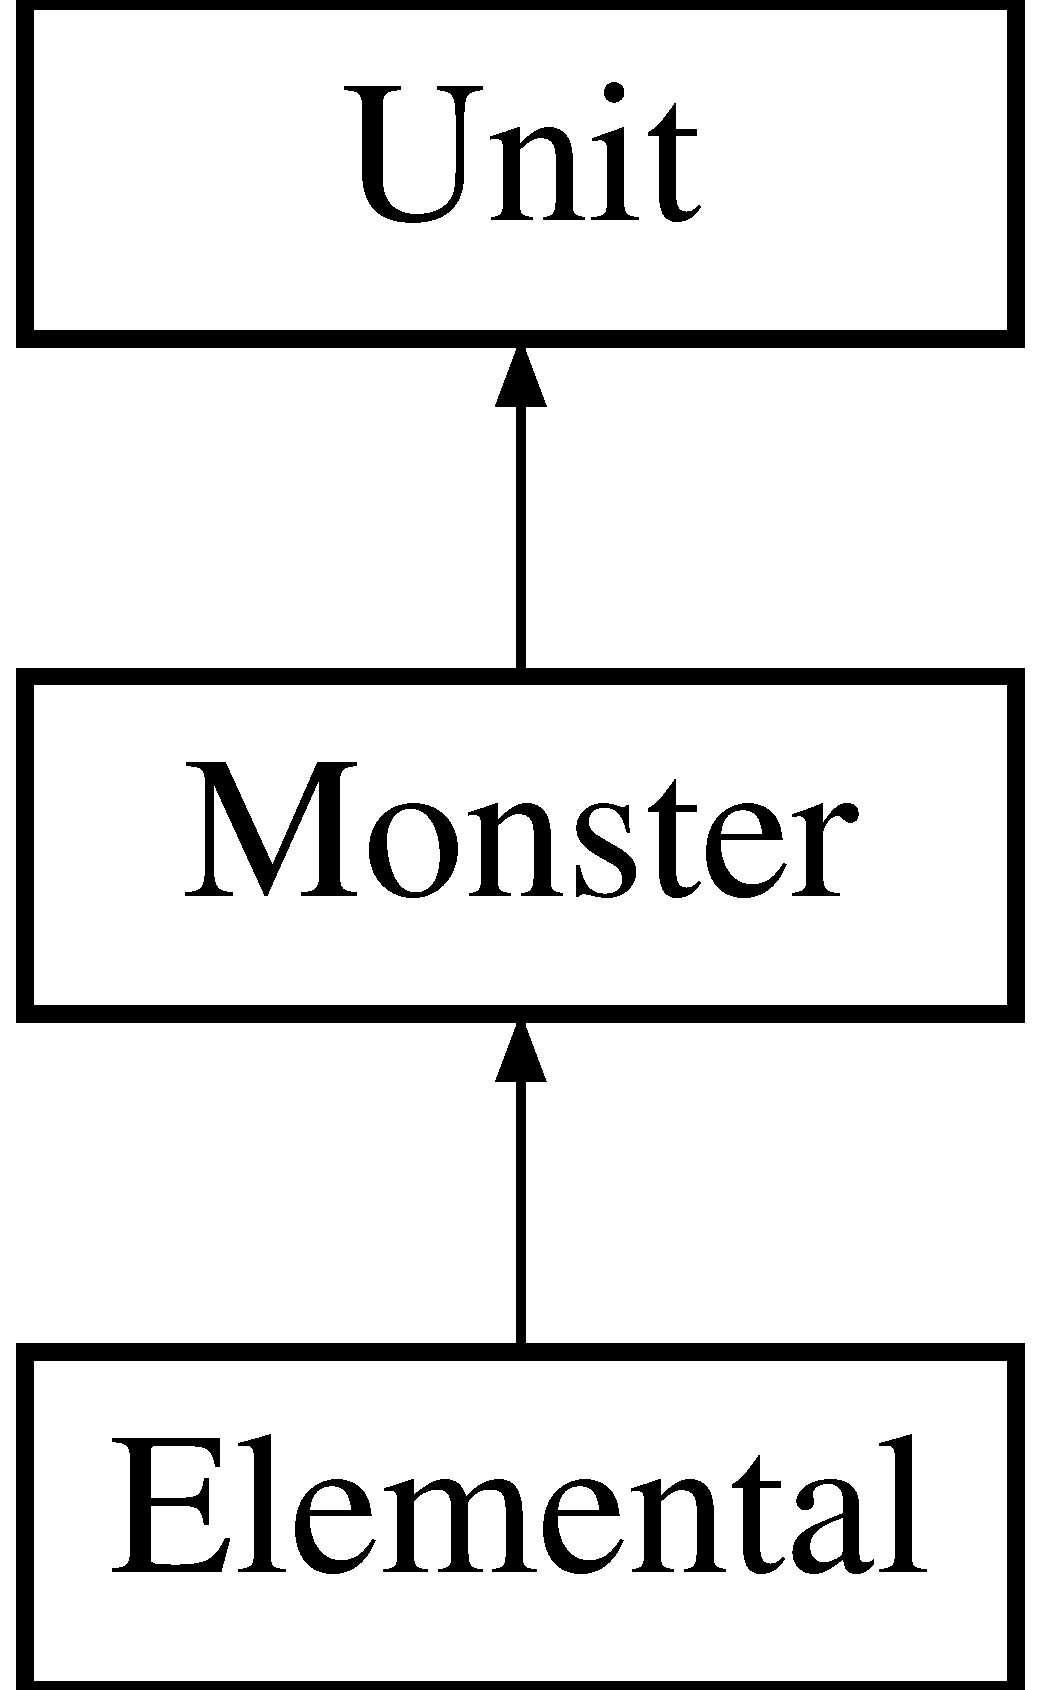
\includegraphics[height=3.000000cm]{class_elemental}
\end{center}
\end{figure}
\subsection*{Public Member Functions}
\begin{DoxyCompactItemize}
\item 
\hyperlink{class_elemental_ab1c090ccbb2ac64d7cd65dbef999d9fb}{Elemental} ()
\end{DoxyCompactItemize}
\subsection*{Additional Inherited Members}


\subsection{Detailed Description}
A concrete \hyperlink{class_unit}{Unit}; Inherits from \hyperlink{class_monster}{Monster}. 

\begin{DoxySeeAlso}{See also}
\hyperlink{class_monster}{Monster} () 
\end{DoxySeeAlso}


\subsection{Constructor \& Destructor Documentation}
\hypertarget{class_elemental_ab1c090ccbb2ac64d7cd65dbef999d9fb}{}\index{Elemental@{Elemental}!Elemental@{Elemental}}
\index{Elemental@{Elemental}!Elemental@{Elemental}}
\subsubsection[{Elemental()}]{\setlength{\rightskip}{0pt plus 5cm}Elemental\+::\+Elemental (
\begin{DoxyParamCaption}
{}
\end{DoxyParamCaption}
)}\label{class_elemental_ab1c090ccbb2ac64d7cd65dbef999d9fb}
Constructor for \hyperlink{class_elemental}{Elemental} class sets the stats and respective \char`\"{}class\char`\"{} of \hyperlink{class_elemental}{Elemental}. 

The documentation for this class was generated from the following files\+:\begin{DoxyCompactItemize}
\item 
Elemental.\+h\item 
Elemental.\+cpp\end{DoxyCompactItemize}

\section{Form Class Reference}
\label{class_form}\index{Form@{Form}}
\subsection*{Public Member Functions}
\begin{DoxyCompactItemize}
\item 
{\bfseries Form} (int input\+Max\+X=300, int input\+Max\+Y=80)\label{class_form_a8e9f65a9142bbecab40c051e2bff4abd}

\item 
void {\bfseries put\+Pixel} (int x, int y)\label{class_form_a56e8191b44ccfdf4e359bb06a6bfc6b5}

\item 
void {\bfseries flush} ()\label{class_form_aaa97c970662093c0936889a5b70b8f04}

\item 
void {\bfseries draw} ()\label{class_form_af2fa46ab3deb4e858bb681e6523a381d}

\end{DoxyCompactItemize}


The documentation for this class was generated from the following file\+:\begin{DoxyCompactItemize}
\item 
Task5(\+Bonus)/Form.\+h\end{DoxyCompactItemize}

\hypertarget{class_goblin}{}\section{Goblin Class Reference}
\label{class_goblin}\index{Goblin@{Goblin}}


A concrete \hyperlink{class_unit}{Unit}; Inherits from \hyperlink{class_monster}{Monster}.  




{\ttfamily \#include $<$Goblin.\+h$>$}

Inheritance diagram for Goblin\+:\begin{figure}[H]
\begin{center}
\leavevmode
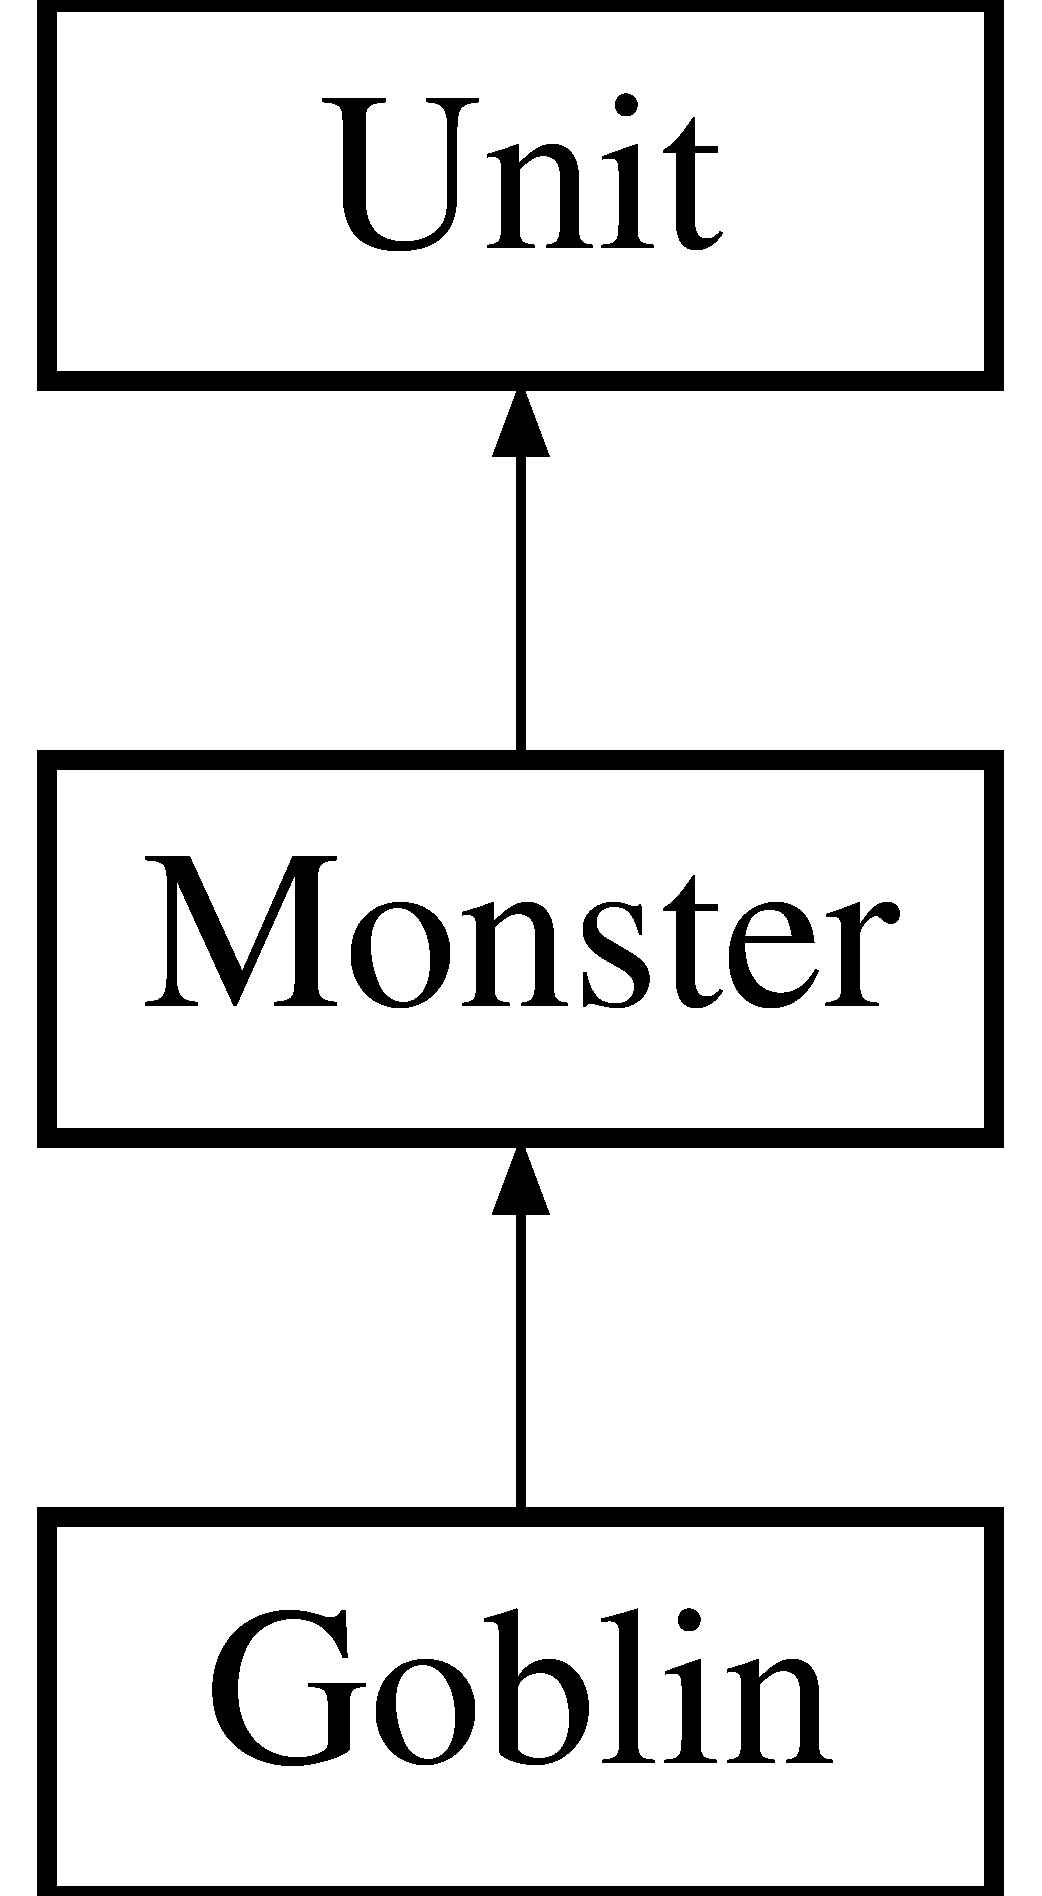
\includegraphics[height=3.000000cm]{class_goblin}
\end{center}
\end{figure}
\subsection*{Public Member Functions}
\begin{DoxyCompactItemize}
\item 
\hyperlink{class_goblin_a22d43a81f99697e13d13a0c56fae9bc4}{Goblin} ()
\end{DoxyCompactItemize}
\subsection*{Additional Inherited Members}


\subsection{Detailed Description}
A concrete \hyperlink{class_unit}{Unit}; Inherits from \hyperlink{class_monster}{Monster}. 

\begin{DoxySeeAlso}{See also}
\hyperlink{class_monster}{Monster} () 
\end{DoxySeeAlso}


\subsection{Constructor \& Destructor Documentation}
\hypertarget{class_goblin_a22d43a81f99697e13d13a0c56fae9bc4}{}\index{Goblin@{Goblin}!Goblin@{Goblin}}
\index{Goblin@{Goblin}!Goblin@{Goblin}}
\subsubsection[{Goblin()}]{\setlength{\rightskip}{0pt plus 5cm}Goblin\+::\+Goblin (
\begin{DoxyParamCaption}
{}
\end{DoxyParamCaption}
)}\label{class_goblin_a22d43a81f99697e13d13a0c56fae9bc4}
Constructor for \hyperlink{class_goblin}{Goblin} class sets the stats and respective \char`\"{}class\char`\"{} of \hyperlink{class_goblin}{Goblin}. 

The documentation for this class was generated from the following files\+:\begin{DoxyCompactItemize}
\item 
Goblin.\+h\item 
Goblin.\+cpp\end{DoxyCompactItemize}

\hypertarget{class_mage}{}\section{Mage Class Reference}
\label{class_mage}\index{Mage@{Mage}}


A concrete \hyperlink{class_unit}{Unit}; Inherits from \hyperlink{class_player}{Player}.  




{\ttfamily \#include $<$Mage.\+h$>$}

Inheritance diagram for Mage\+:\begin{figure}[H]
\begin{center}
\leavevmode
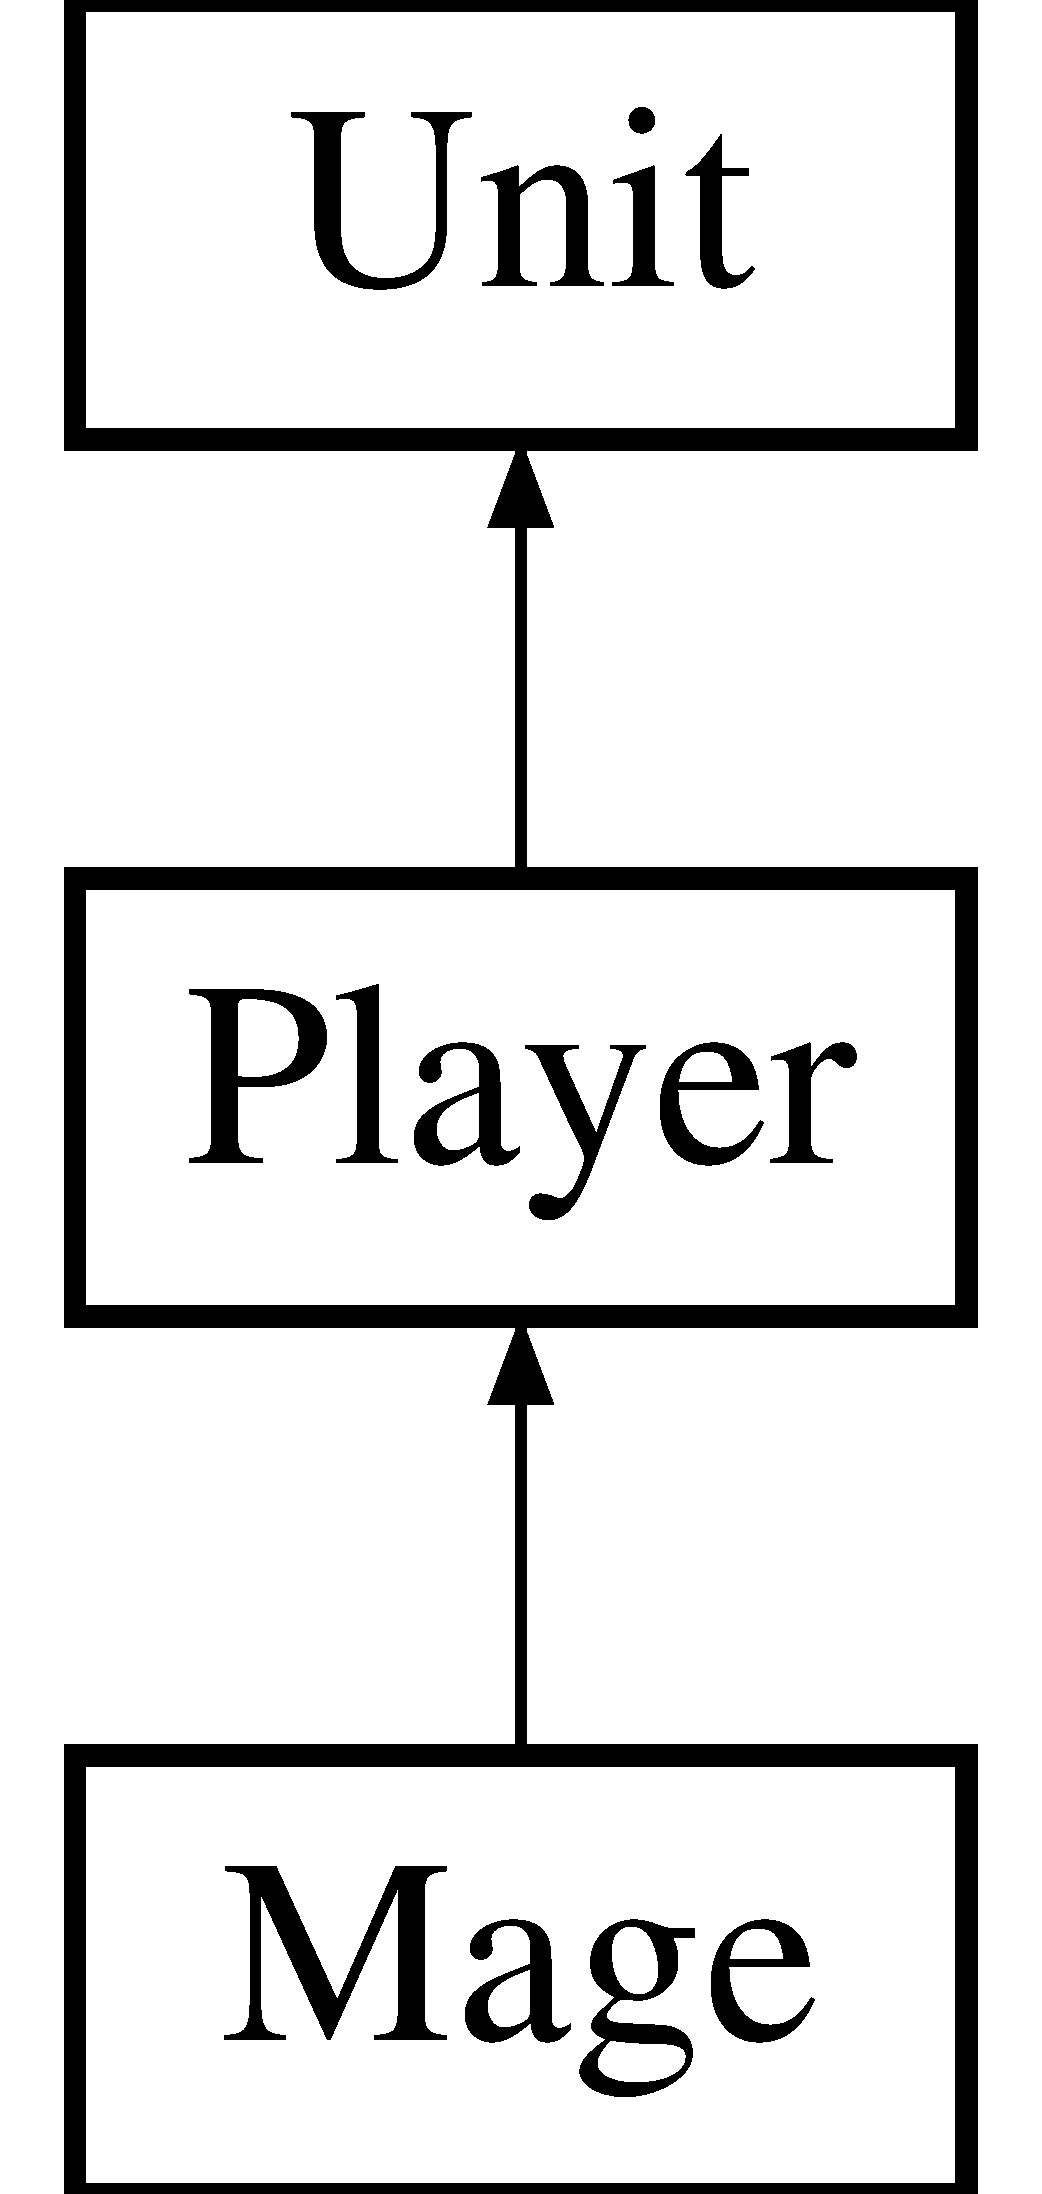
\includegraphics[height=3.000000cm]{class_mage}
\end{center}
\end{figure}
\subsection*{Public Member Functions}
\begin{DoxyCompactItemize}
\item 
\hyperlink{class_mage_a9d7d4455a6fa1f8e35117e0dc301d082}{Mage} ()
\end{DoxyCompactItemize}
\subsection*{Additional Inherited Members}


\subsection{Detailed Description}
A concrete \hyperlink{class_unit}{Unit}; Inherits from \hyperlink{class_player}{Player}. 

\begin{DoxySeeAlso}{See also}
\hyperlink{class_player}{Player} () 
\end{DoxySeeAlso}


\subsection{Constructor \& Destructor Documentation}
\hypertarget{class_mage_a9d7d4455a6fa1f8e35117e0dc301d082}{}\index{Mage@{Mage}!Mage@{Mage}}
\index{Mage@{Mage}!Mage@{Mage}}
\subsubsection[{Mage()}]{\setlength{\rightskip}{0pt plus 5cm}Mage\+::\+Mage (
\begin{DoxyParamCaption}
{}
\end{DoxyParamCaption}
)}\label{class_mage_a9d7d4455a6fa1f8e35117e0dc301d082}
Constructor for \hyperlink{class_mage}{Mage} class sets the stats and respective \char`\"{}class\char`\"{} of \hyperlink{class_mage}{Mage}. 

The documentation for this class was generated from the following files\+:\begin{DoxyCompactItemize}
\item 
Mage.\+h\item 
Mage.\+cpp\end{DoxyCompactItemize}

\hypertarget{class_magic_factory}{}\section{Magic\+Factory Class Reference}
\label{class_magic_factory}\index{Magic\+Factory@{Magic\+Factory}}


Concrete Factory that creates a \hyperlink{class_mage}{Mage} or \hyperlink{class_elemental}{Elemental} object.  




{\ttfamily \#include $<$Magic\+Factory.\+h$>$}

Inheritance diagram for Magic\+Factory\+:\begin{figure}[H]
\begin{center}
\leavevmode
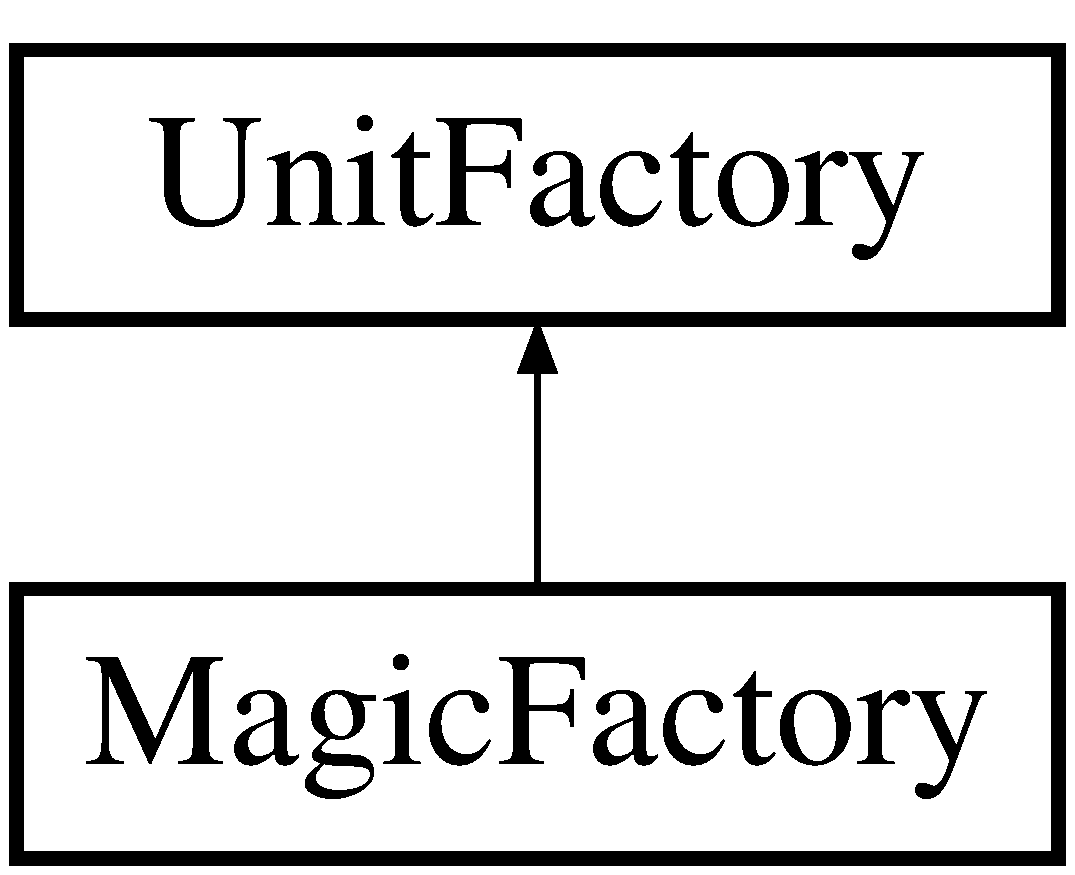
\includegraphics[height=2.000000cm]{class_magic_factory}
\end{center}
\end{figure}
\subsection*{Public Member Functions}
\begin{DoxyCompactItemize}
\item 
\hypertarget{class_magic_factory_a3021b979bd991e32e311c8869d500b46}{}virtual \hyperlink{class_unit}{Unit} $\ast$ \hyperlink{class_magic_factory_a3021b979bd991e32e311c8869d500b46}{create\+Player} ()\label{class_magic_factory_a3021b979bd991e32e311c8869d500b46}

\begin{DoxyCompactList}\small\item\em Concrete implementation of create\+Player, will create a \hyperlink{class_mage}{Mage}. \end{DoxyCompactList}\item 
\hypertarget{class_magic_factory_aaef72871585cca14e5b847fc44ce3c2b}{}virtual \hyperlink{class_unit}{Unit} $\ast$ \hyperlink{class_magic_factory_aaef72871585cca14e5b847fc44ce3c2b}{create\+Monster} ()\label{class_magic_factory_aaef72871585cca14e5b847fc44ce3c2b}

\begin{DoxyCompactList}\small\item\em Concrete impletation of create\+Monster, will create an \hyperlink{class_elemental}{Elemental}. \end{DoxyCompactList}\end{DoxyCompactItemize}
\subsection*{Additional Inherited Members}


\subsection{Detailed Description}
Concrete Factory that creates a \hyperlink{class_mage}{Mage} or \hyperlink{class_elemental}{Elemental} object. 

\begin{DoxySeeAlso}{See also}
\hyperlink{class_unit_factory}{Unit\+Factory} 
\end{DoxySeeAlso}


The documentation for this class was generated from the following files\+:\begin{DoxyCompactItemize}
\item 
Magic\+Factory.\+h\item 
Magic\+Factory.\+cpp\end{DoxyCompactItemize}

\hypertarget{class_monster}{}\section{Monster Class Reference}
\label{class_monster}\index{Monster@{Monster}}


Is the class from which all concrete Monsters derive inherites from \hyperlink{class_unit}{Unit}.  




{\ttfamily \#include $<$Monster.\+h$>$}

Inheritance diagram for Monster\+:\begin{figure}[H]
\begin{center}
\leavevmode
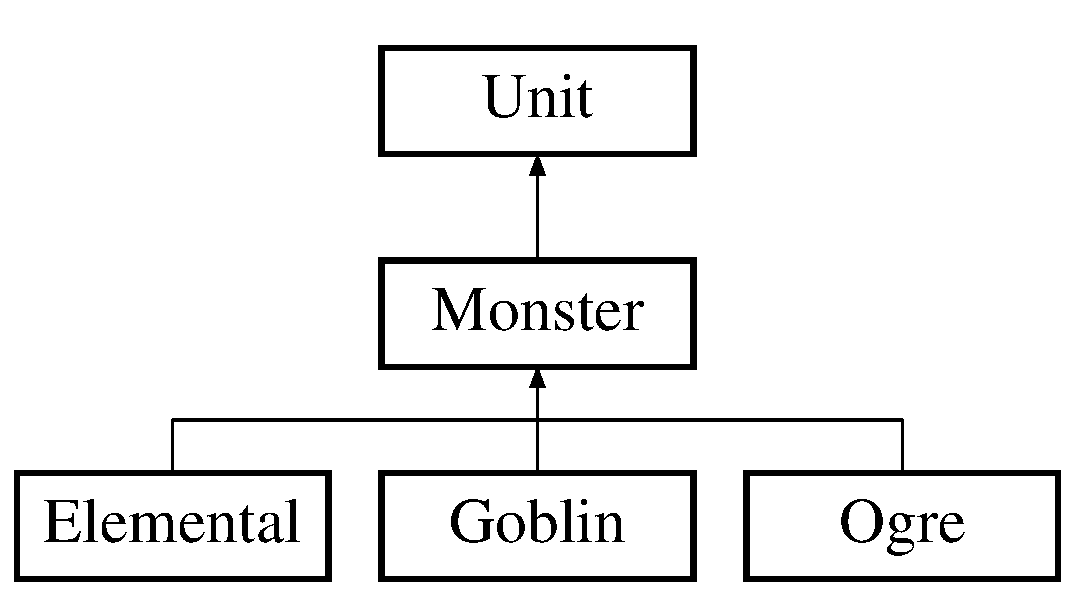
\includegraphics[height=3.000000cm]{class_monster}
\end{center}
\end{figure}
\subsection*{Public Member Functions}
\begin{DoxyCompactItemize}
\item 
\hyperlink{class_unit}{Unit} $\ast$ \hyperlink{class_monster_a1ee9cabba47d15d4e196d19561250ee0}{clone} ()
\begin{DoxyCompactList}\small\item\em Implementation of inherited virtual function. \end{DoxyCompactList}\end{DoxyCompactItemize}
\subsection*{Additional Inherited Members}


\subsection{Detailed Description}
Is the class from which all concrete Monsters derive inherites from \hyperlink{class_unit}{Unit}. 

\begin{DoxySeeAlso}{See also}
\hyperlink{class_unit}{Unit} 
\end{DoxySeeAlso}


\subsection{Member Function Documentation}
\hypertarget{class_monster_a1ee9cabba47d15d4e196d19561250ee0}{}\index{Monster@{Monster}!clone@{clone}}
\index{clone@{clone}!Monster@{Monster}}
\subsubsection[{clone()}]{\setlength{\rightskip}{0pt plus 5cm}{\bf Unit} $\ast$ Monster\+::clone (
\begin{DoxyParamCaption}
{}
\end{DoxyParamCaption}
)\hspace{0.3cm}{\ttfamily [virtual]}}\label{class_monster_a1ee9cabba47d15d4e196d19561250ee0}


Implementation of inherited virtual function. 

\begin{DoxyReturn}{Returns}
Unit$\ast$ containing a deep copy of this object. 
\end{DoxyReturn}


Implements \hyperlink{class_unit_add809c0669cb6b08afae913da60c4cc1}{Unit}.



The documentation for this class was generated from the following files\+:\begin{DoxyCompactItemize}
\item 
Monster.\+h\item 
Monster.\+cpp\end{DoxyCompactItemize}

\hypertarget{class_ogre}{}\section{Ogre Class Reference}
\label{class_ogre}\index{Ogre@{Ogre}}


A concrete \hyperlink{class_unit}{Unit}; Inherits from \hyperlink{class_monster}{Monster}.  




{\ttfamily \#include $<$Ogre.\+h$>$}

Inheritance diagram for Ogre\+:\begin{figure}[H]
\begin{center}
\leavevmode
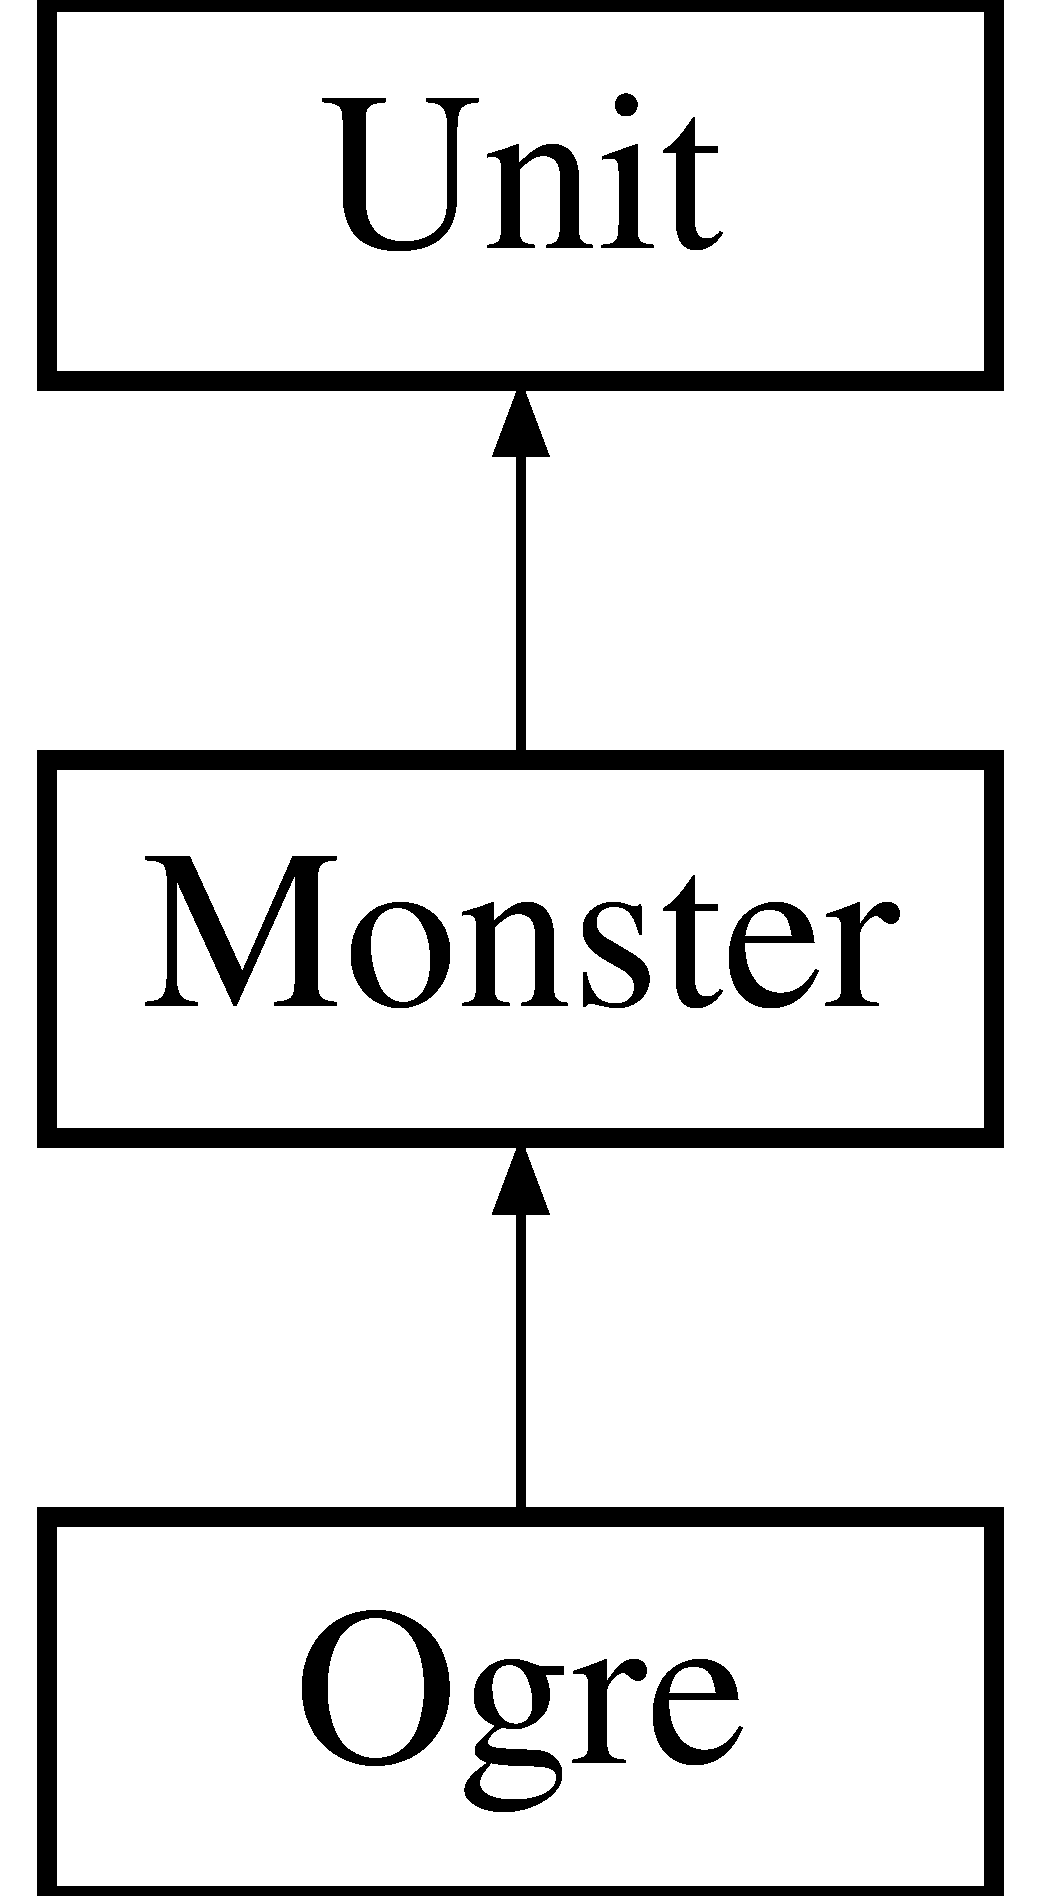
\includegraphics[height=3.000000cm]{class_ogre}
\end{center}
\end{figure}
\subsection*{Public Member Functions}
\begin{DoxyCompactItemize}
\item 
\hyperlink{class_ogre_aeb7c78cfd86de3a8e2175d87dac17c9f}{Ogre} ()
\end{DoxyCompactItemize}
\subsection*{Additional Inherited Members}


\subsection{Detailed Description}
A concrete \hyperlink{class_unit}{Unit}; Inherits from \hyperlink{class_monster}{Monster}. 

\begin{DoxySeeAlso}{See also}
\hyperlink{class_monster}{Monster} () 
\end{DoxySeeAlso}


\subsection{Constructor \& Destructor Documentation}
\hypertarget{class_ogre_aeb7c78cfd86de3a8e2175d87dac17c9f}{}\index{Ogre@{Ogre}!Ogre@{Ogre}}
\index{Ogre@{Ogre}!Ogre@{Ogre}}
\subsubsection[{Ogre()}]{\setlength{\rightskip}{0pt plus 5cm}Ogre\+::\+Ogre (
\begin{DoxyParamCaption}
{}
\end{DoxyParamCaption}
)}\label{class_ogre_aeb7c78cfd86de3a8e2175d87dac17c9f}
Constructor for \hyperlink{class_ogre}{Ogre} class sets the stats and respective \char`\"{}class\char`\"{} of Orgre. 

The documentation for this class was generated from the following files\+:\begin{DoxyCompactItemize}
\item 
Ogre.\+h\item 
Ogre.\+cpp\end{DoxyCompactItemize}

\hypertarget{class_piercing_factory}{}\section{Piercing\+Factory Class Reference}
\label{class_piercing_factory}\index{Piercing\+Factory@{Piercing\+Factory}}


Concrete factory that creates \hyperlink{class_thief}{Thief} or \hyperlink{class_goblin}{Goblin} objects.  




{\ttfamily \#include $<$Piercing\+Factory.\+h$>$}

Inheritance diagram for Piercing\+Factory\+:\begin{figure}[H]
\begin{center}
\leavevmode
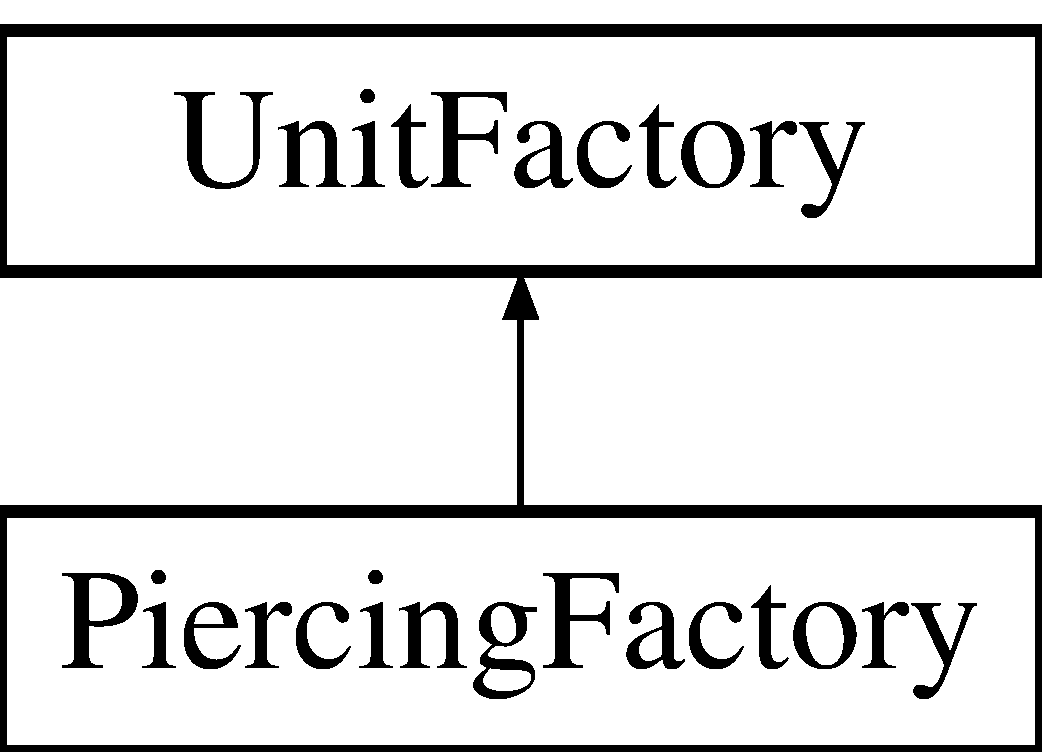
\includegraphics[height=2.000000cm]{class_piercing_factory}
\end{center}
\end{figure}
\subsection*{Public Member Functions}
\begin{DoxyCompactItemize}
\item 
\hypertarget{class_piercing_factory_a3a2f3736e85a5c4b0ad0160b1b34d796}{}virtual \hyperlink{class_unit}{Unit} $\ast$ \hyperlink{class_piercing_factory_a3a2f3736e85a5c4b0ad0160b1b34d796}{create\+Player} ()\label{class_piercing_factory_a3a2f3736e85a5c4b0ad0160b1b34d796}

\begin{DoxyCompactList}\small\item\em Concrete implementation of create\+Player, will create a Theif. \end{DoxyCompactList}\item 
\hypertarget{class_piercing_factory_a042235a24b114b8b66e3e7733109e504}{}virtual \hyperlink{class_unit}{Unit} $\ast$ \hyperlink{class_piercing_factory_a042235a24b114b8b66e3e7733109e504}{create\+Monster} ()\label{class_piercing_factory_a042235a24b114b8b66e3e7733109e504}

\begin{DoxyCompactList}\small\item\em Concrete impletation of create\+Monster, will create a \hyperlink{class_goblin}{Goblin}. \end{DoxyCompactList}\end{DoxyCompactItemize}
\subsection*{Additional Inherited Members}


\subsection{Detailed Description}
Concrete factory that creates \hyperlink{class_thief}{Thief} or \hyperlink{class_goblin}{Goblin} objects. 

\begin{DoxySeeAlso}{See also}
\hyperlink{class_unit_factory}{Unit\+Factory} 
\end{DoxySeeAlso}


The documentation for this class was generated from the following files\+:\begin{DoxyCompactItemize}
\item 
Piercing\+Factory.\+h\item 
Piercing\+Factory.\+cpp\end{DoxyCompactItemize}

\section{Player Class Reference}
\label{class_player}\index{Player@{Player}}


Is the class from which all concrete Monsters derive inherites from \doxyref{Unit}{p.}{class_unit}.  




{\ttfamily \#include $<$Player.\+h$>$}

Inheritance diagram for Player\+:\begin{figure}[H]
\begin{center}
\leavevmode
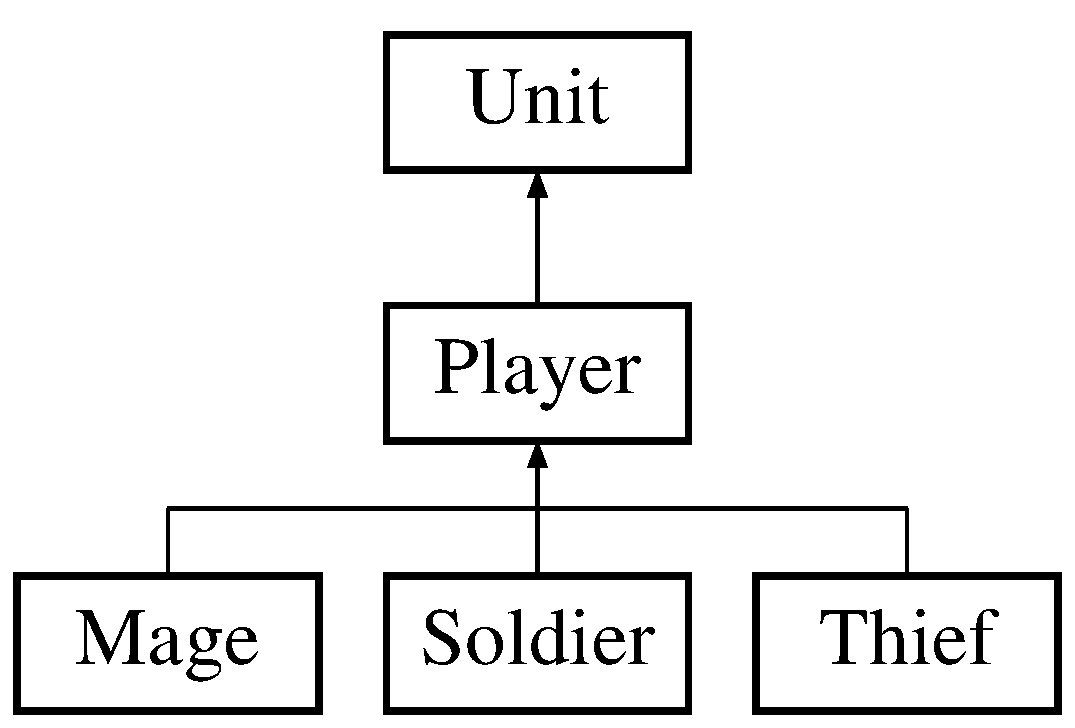
\includegraphics[height=3.000000cm]{class_player}
\end{center}
\end{figure}
\subsection*{Public Member Functions}
\begin{DoxyCompactItemize}
\item 
{\bf Unit} $\ast$ {\bf clone} ()
\begin{DoxyCompactList}\small\item\em Implementation of inherited virtual function. \end{DoxyCompactList}\item 
void {\bf attack} ({\bf Unit} \&input\+Unit)\label{class_player_a6227fdb9ebd053540582793c0d91effa}

\begin{DoxyCompactList}\small\item\em Implementation of inherited virtual function. \end{DoxyCompactList}\end{DoxyCompactItemize}
\subsection*{Additional Inherited Members}


\subsection{Detailed Description}
Is the class from which all concrete Monsters derive inherites from \doxyref{Unit}{p.}{class_unit}. 

\begin{DoxySeeAlso}{See also}
\doxyref{Unit}{p.}{class_unit} 
\end{DoxySeeAlso}


\subsection{Member Function Documentation}
\index{Player@{Player}!clone@{clone}}
\index{clone@{clone}!Player@{Player}}
\subsubsection[{clone()}]{\setlength{\rightskip}{0pt plus 5cm}{\bf Unit} $\ast$ Player\+::clone (
\begin{DoxyParamCaption}
{}
\end{DoxyParamCaption}
)\hspace{0.3cm}{\ttfamily [virtual]}}\label{class_player_ad690ac4f9f851298abeb0955321ea29e}


Implementation of inherited virtual function. 

\begin{DoxyReturn}{Returns}
Unit$\ast$ containing a deep copy of this object. 
\end{DoxyReturn}


Implements {\bf Unit} \doxyref{}{p.}{class_unit_add809c0669cb6b08afae913da60c4cc1}.



The documentation for this class was generated from the following files\+:\begin{DoxyCompactItemize}
\item 
Player.\+h\item 
Player.\+cpp\end{DoxyCompactItemize}

\hypertarget{class_soldier}{}\section{Soldier Class Reference}
\label{class_soldier}\index{Soldier@{Soldier}}


A concrete \hyperlink{class_unit}{Unit}; Inherits from \hyperlink{class_player}{Player}.  




{\ttfamily \#include $<$Soldier.\+h$>$}

Inheritance diagram for Soldier\+:\begin{figure}[H]
\begin{center}
\leavevmode
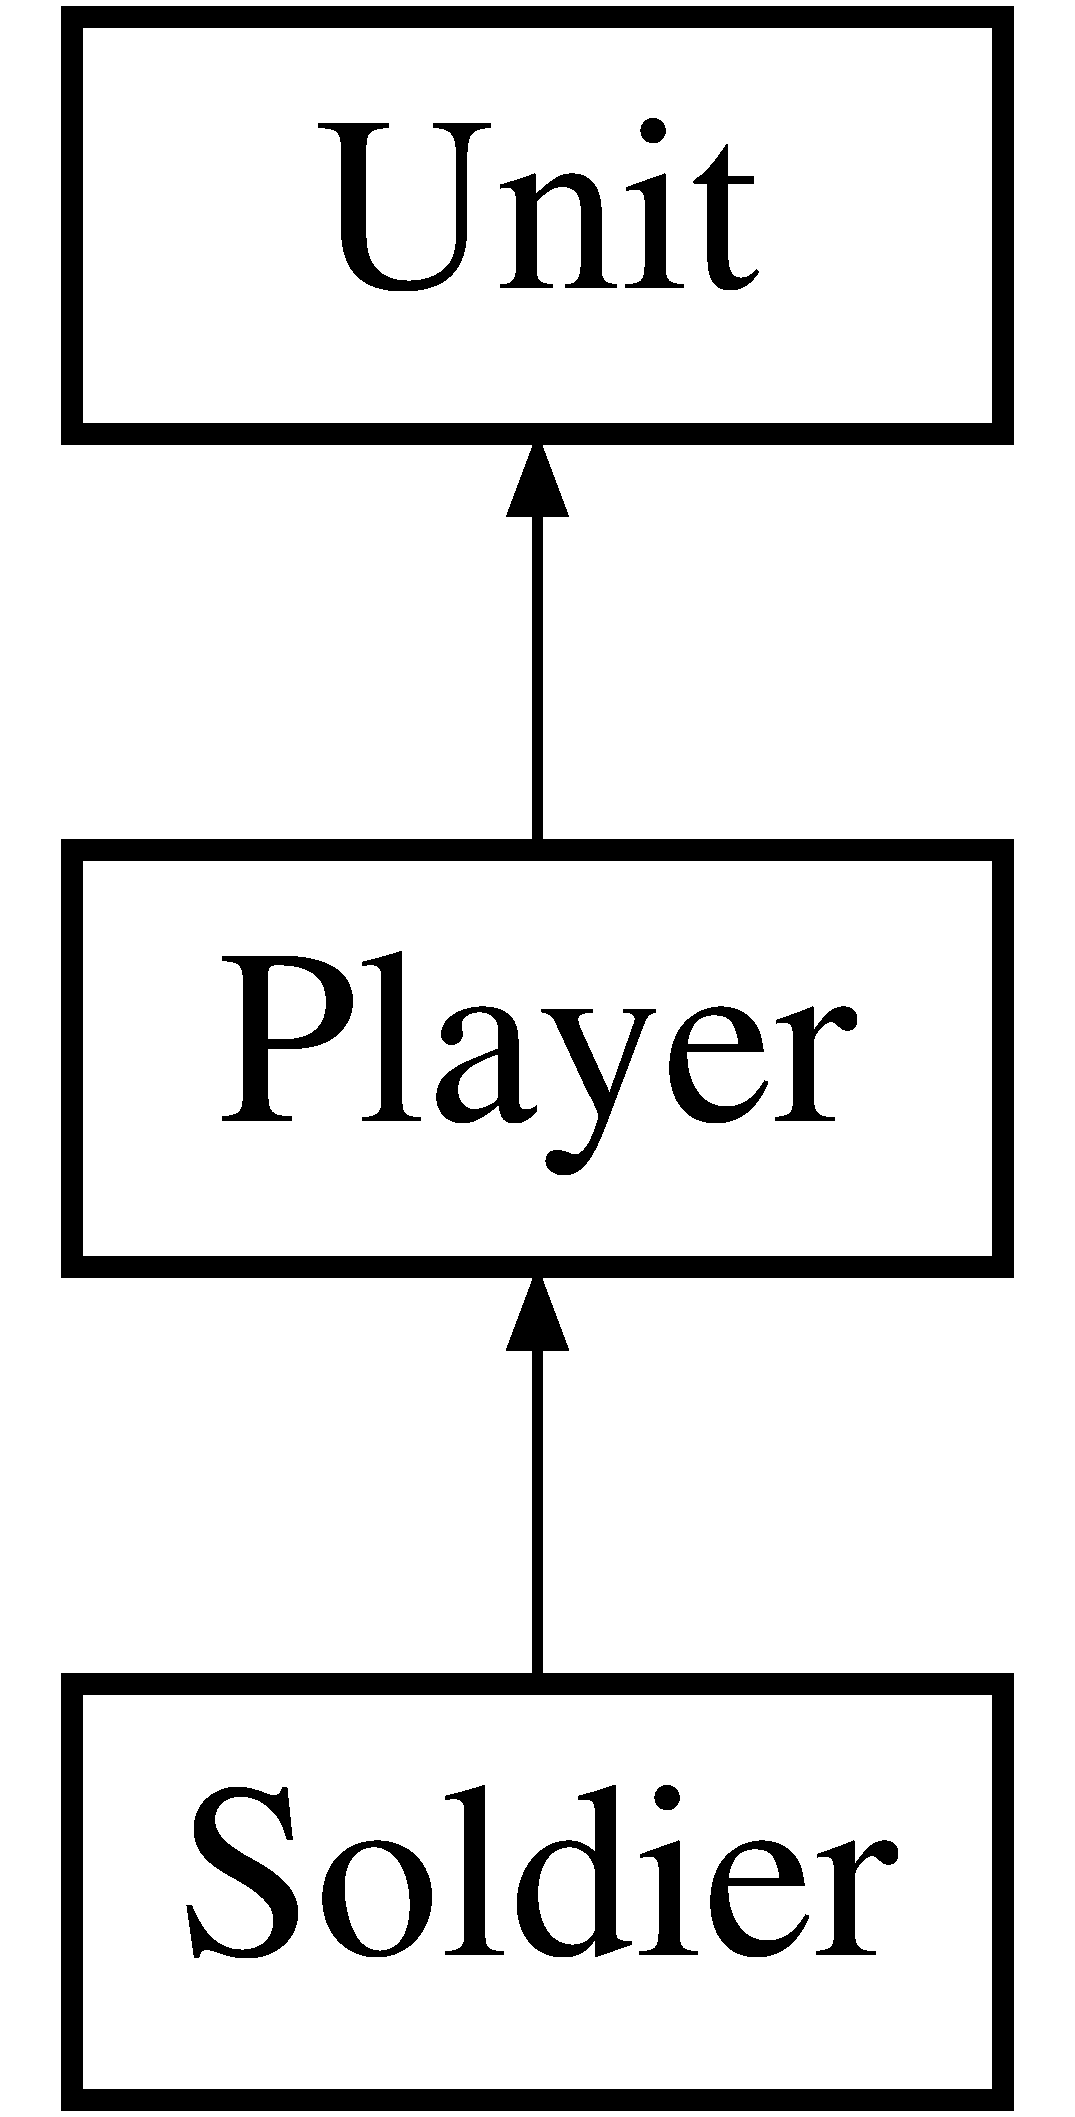
\includegraphics[height=3.000000cm]{class_soldier}
\end{center}
\end{figure}
\subsection*{Public Member Functions}
\begin{DoxyCompactItemize}
\item 
\hyperlink{class_soldier_ad3144b22a146ef85eaff30a2a5ab78c0}{Soldier} ()
\end{DoxyCompactItemize}
\subsection*{Additional Inherited Members}


\subsection{Detailed Description}
A concrete \hyperlink{class_unit}{Unit}; Inherits from \hyperlink{class_player}{Player}. 

\begin{DoxySeeAlso}{See also}
\hyperlink{class_player}{Player} () 
\end{DoxySeeAlso}


\subsection{Constructor \& Destructor Documentation}
\hypertarget{class_soldier_ad3144b22a146ef85eaff30a2a5ab78c0}{}\index{Soldier@{Soldier}!Soldier@{Soldier}}
\index{Soldier@{Soldier}!Soldier@{Soldier}}
\subsubsection[{Soldier()}]{\setlength{\rightskip}{0pt plus 5cm}Soldier\+::\+Soldier (
\begin{DoxyParamCaption}
{}
\end{DoxyParamCaption}
)}\label{class_soldier_ad3144b22a146ef85eaff30a2a5ab78c0}
Constructor for \hyperlink{class_soldier}{Soldier} class sets the stats and respective \char`\"{}class\char`\"{} of \hyperlink{class_soldier}{Soldier}. 

The documentation for this class was generated from the following files\+:\begin{DoxyCompactItemize}
\item 
Soldier.\+h\item 
Soldier.\+cpp\end{DoxyCompactItemize}

\section{Thief Class Reference}
\label{class_thief}\index{Thief@{Thief}}


A concrete \doxyref{Unit}{p.}{class_unit}; Inherits from \doxyref{Player}{p.}{class_player}.  




{\ttfamily \#include $<$Thief.\+h$>$}

Inheritance diagram for Thief\+:\begin{figure}[H]
\begin{center}
\leavevmode
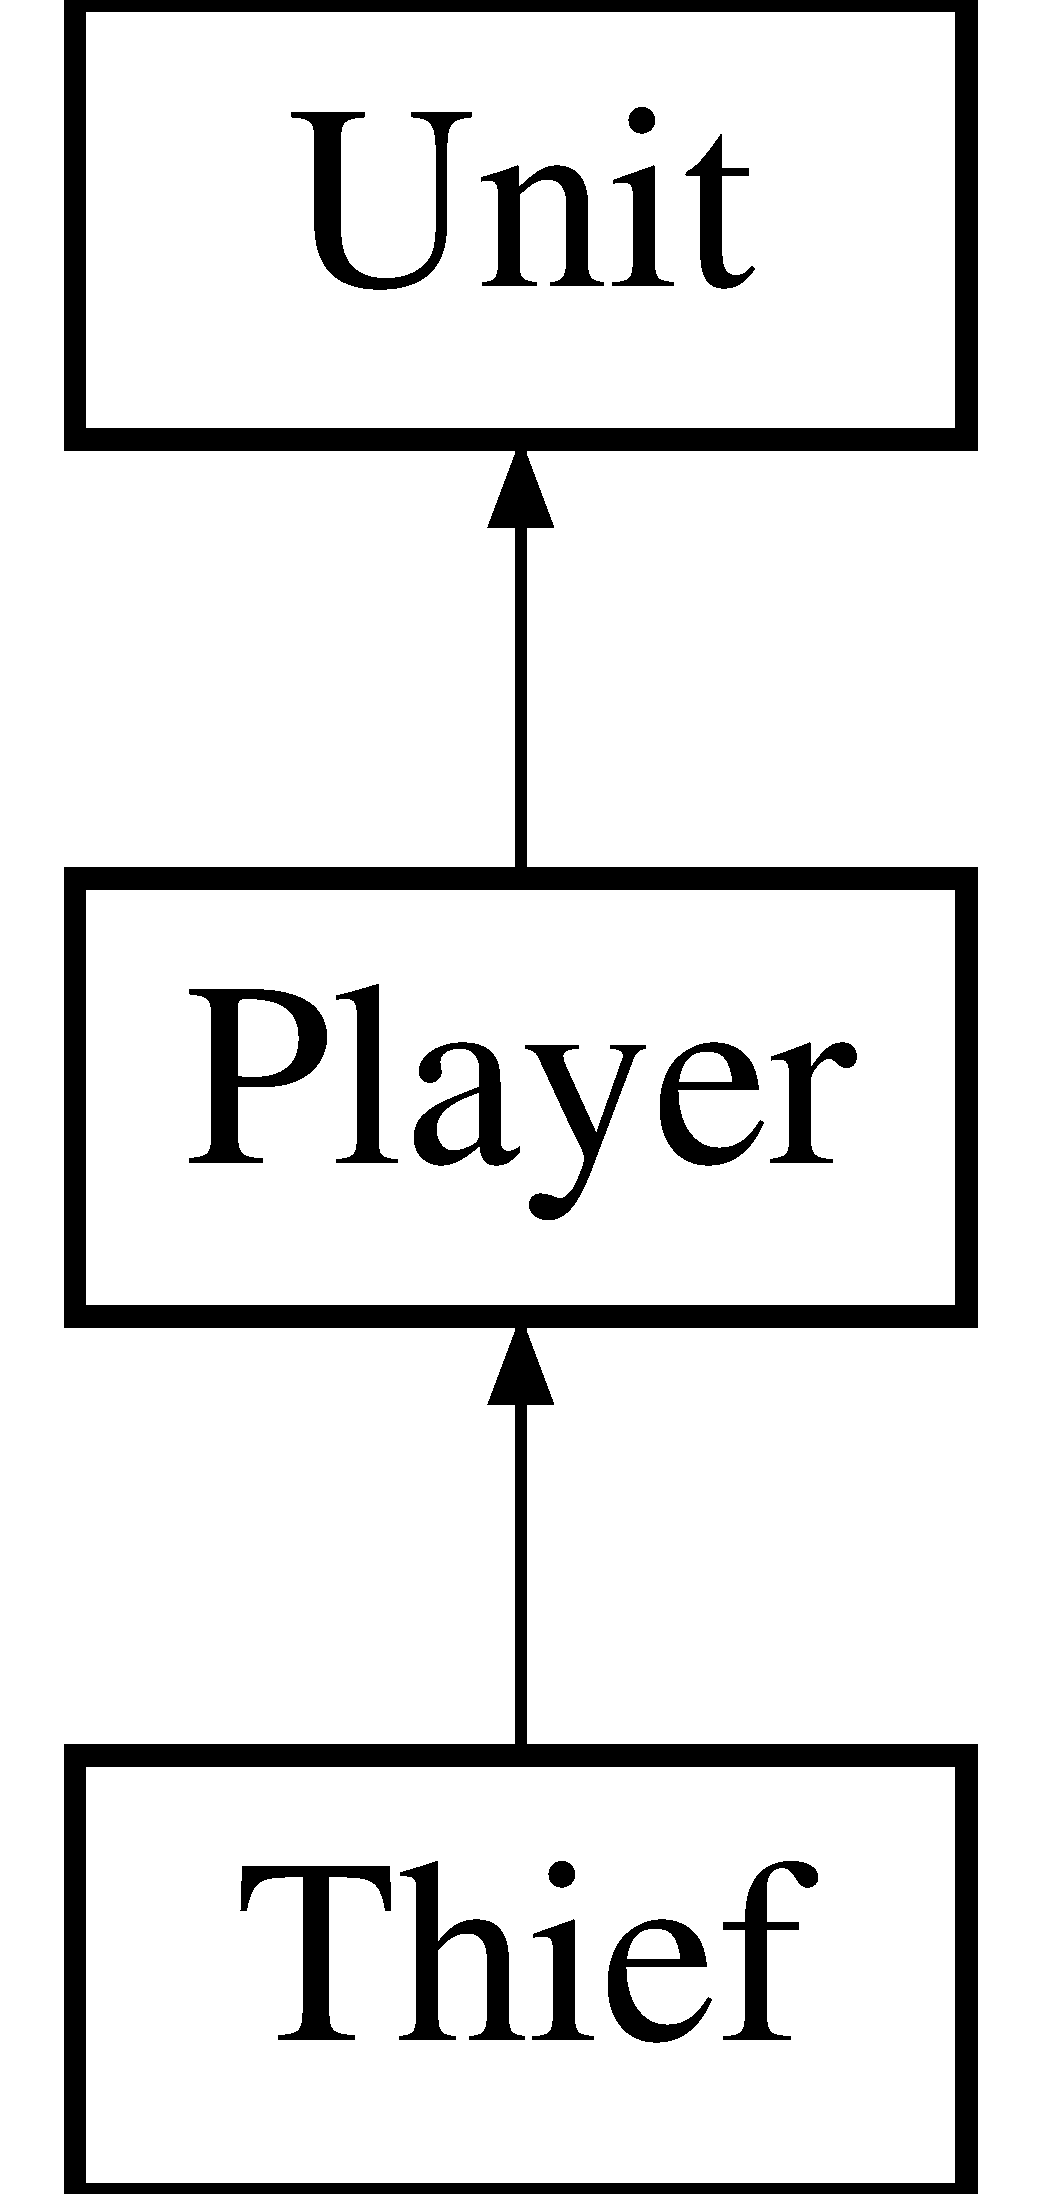
\includegraphics[height=3.000000cm]{class_thief}
\end{center}
\end{figure}
\subsection*{Public Member Functions}
\begin{DoxyCompactItemize}
\item 
{\bf Thief} ()
\end{DoxyCompactItemize}
\subsection*{Additional Inherited Members}


\subsection{Detailed Description}
A concrete \doxyref{Unit}{p.}{class_unit}; Inherits from \doxyref{Player}{p.}{class_player}. 

\begin{DoxySeeAlso}{See also}
\doxyref{Player}{p.}{class_player} () 
\end{DoxySeeAlso}


\subsection{Constructor \& Destructor Documentation}
\index{Thief@{Thief}!Thief@{Thief}}
\index{Thief@{Thief}!Thief@{Thief}}
\subsubsection[{Thief()}]{\setlength{\rightskip}{0pt plus 5cm}Thief\+::\+Thief (
\begin{DoxyParamCaption}
{}
\end{DoxyParamCaption}
)}\label{class_thief_aa27752dd9c628bf41d297fedee59c2df}
Constructor for \doxyref{Thief}{p.}{class_thief} class sets the stats and respective \char`\"{}class\char`\"{} of \doxyref{Thief}{p.}{class_thief}. 

The documentation for this class was generated from the following files\+:\begin{DoxyCompactItemize}
\item 
Thief.\+h\item 
Thief.\+cpp\end{DoxyCompactItemize}

\section{Unit Class Reference}
\label{class_unit}\index{Unit@{Unit}}


Is the class from which all concrete Units derive.  




{\ttfamily \#include $<$Unit.\+h$>$}

Inheritance diagram for Unit\+:\begin{figure}[H]
\begin{center}
\leavevmode
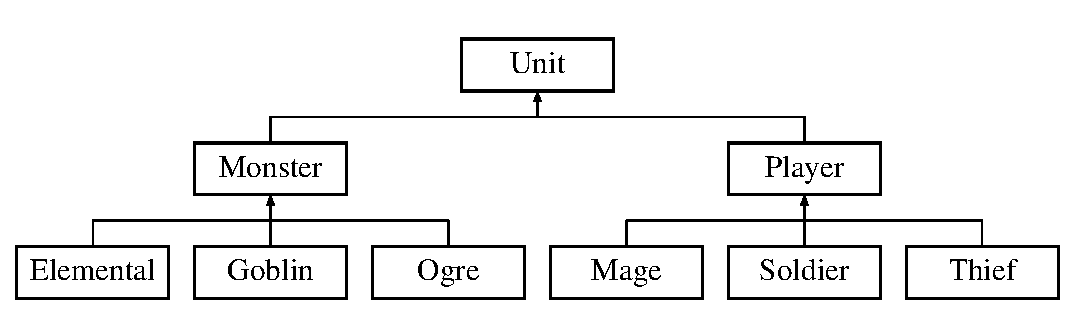
\includegraphics[height=3.000000cm]{class_unit}
\end{center}
\end{figure}
\subsection*{Public Member Functions}
\begin{DoxyCompactItemize}
\item 
virtual {\bf $\sim$\+Unit} ()\label{class_unit_a6353fc4c0a329997ad4abcf0dcb4eb27}

\begin{DoxyCompactList}\small\item\em virtual destructor \end{DoxyCompactList}\item 
virtual {\bf Unit} $\ast$ {\bf clone} ()=0
\begin{DoxyCompactList}\small\item\em pure virtual function that allows prototypes of Units to be clone. \end{DoxyCompactList}\item 
virtual void {\bf attack} ({\bf Unit} \&input\+Unit)=0
\begin{DoxyCompactList}\small\item\em pure virtual function that allows prototypes of Units to be clone. \end{DoxyCompactList}\item 
int {\bf get\+Damage} ()
\begin{DoxyCompactList}\small\item\em Public interface to damage member variable. \end{DoxyCompactList}\item 
int {\bf get\+Health} ()
\begin{DoxyCompactList}\small\item\em Public interface to health member variable. \end{DoxyCompactList}\item 
string {\bf get\+Class} ()
\begin{DoxyCompactList}\small\item\em Public interface to \char`\"{}class\char`\"{} member variable. \end{DoxyCompactList}\end{DoxyCompactItemize}
\subsection*{Protected Member Functions}
\begin{DoxyCompactItemize}
\item 
void {\bf set\+Damage} (int input\+Damage)\label{class_unit_ac57bb8bbddb45b4b55f841e43f96fe0b}

\begin{DoxyCompactList}\small\item\em Protected interface to modify damage member. \end{DoxyCompactList}\item 
void {\bf set\+Health} (int input\+Health)\label{class_unit_ac763191e46e663938479a9be72c5bd39}

\begin{DoxyCompactList}\small\item\em Protected interface to modify health member. \end{DoxyCompactList}\item 
void {\bf set\+Class} (string input\+Class)\label{class_unit_a0da561786edca63a3282b60a1203ef61}

\begin{DoxyCompactList}\small\item\em Protected interface to modify \char`\"{}class\char`\"{} member. \end{DoxyCompactList}\end{DoxyCompactItemize}
\subsection*{Protected Attributes}
\begin{DoxyCompactItemize}
\item 
string {\bfseries unit\+Class}\label{class_unit_a0d8686cf27c3054dff4d0961cb3142d6}

\item 
int {\bfseries damage}\label{class_unit_a92bfb1430ab13e69d4c703a7fc8bafdb}

\item 
int {\bfseries health}\label{class_unit_aa0d11313f047316fc48c7b523d2fc206}

\end{DoxyCompactItemize}


\subsection{Detailed Description}
Is the class from which all concrete Units derive. 

\subsection{Member Function Documentation}
\index{Unit@{Unit}!attack@{attack}}
\index{attack@{attack}!Unit@{Unit}}
\subsubsection[{attack(\+Unit \&input\+Unit)=0}]{\setlength{\rightskip}{0pt plus 5cm}virtual void Unit\+::attack (
\begin{DoxyParamCaption}
\item[{{\bf Unit} \&}]{input\+Unit}
\end{DoxyParamCaption}
)\hspace{0.3cm}{\ttfamily [pure virtual]}}\label{class_unit_afdd0519bfbdd92edb38be1e14bafbca5}


pure virtual function that allows prototypes of Units to be clone. 

\begin{DoxyReturn}{Returns}
a new \doxyref{Unit}{p.}{class_unit} cloned from member variables. 
\end{DoxyReturn}


Implemented in {\bf Monster} \doxyref{}{p.}{class_monster_a390b3ab1a26e3c3e79d65ad4815e252b}, and {\bf Player} \doxyref{}{p.}{class_player_a6227fdb9ebd053540582793c0d91effa}.

\index{Unit@{Unit}!clone@{clone}}
\index{clone@{clone}!Unit@{Unit}}
\subsubsection[{clone()=0}]{\setlength{\rightskip}{0pt plus 5cm}virtual {\bf Unit}$\ast$ Unit\+::clone (
\begin{DoxyParamCaption}
{}
\end{DoxyParamCaption}
)\hspace{0.3cm}{\ttfamily [pure virtual]}}\label{class_unit_add809c0669cb6b08afae913da60c4cc1}


pure virtual function that allows prototypes of Units to be clone. 

\begin{DoxyReturn}{Returns}
a new \doxyref{Unit}{p.}{class_unit} cloned from member variables. 
\end{DoxyReturn}


Implemented in {\bf Monster} \doxyref{}{p.}{class_monster_a1ee9cabba47d15d4e196d19561250ee0}, and {\bf Player} \doxyref{}{p.}{class_player_ad690ac4f9f851298abeb0955321ea29e}.

\index{Unit@{Unit}!get\+Class@{get\+Class}}
\index{get\+Class@{get\+Class}!Unit@{Unit}}
\subsubsection[{get\+Class()}]{\setlength{\rightskip}{0pt plus 5cm}string Unit\+::get\+Class (
\begin{DoxyParamCaption}
{}
\end{DoxyParamCaption}
)}\label{class_unit_a4c4dde0419950aa3b44302bbff2af810}


Public interface to \char`\"{}class\char`\"{} member variable. 

\begin{DoxyReturn}{Returns}
string containing the class of object. 
\end{DoxyReturn}
\index{Unit@{Unit}!get\+Damage@{get\+Damage}}
\index{get\+Damage@{get\+Damage}!Unit@{Unit}}
\subsubsection[{get\+Damage()}]{\setlength{\rightskip}{0pt plus 5cm}int Unit\+::get\+Damage (
\begin{DoxyParamCaption}
{}
\end{DoxyParamCaption}
)}\label{class_unit_a7b0dbed96660669a2234b715018781fa}


Public interface to damage member variable. 

\begin{DoxyReturn}{Returns}
int containing value of damage. 
\end{DoxyReturn}
\index{Unit@{Unit}!get\+Health@{get\+Health}}
\index{get\+Health@{get\+Health}!Unit@{Unit}}
\subsubsection[{get\+Health()}]{\setlength{\rightskip}{0pt plus 5cm}int Unit\+::get\+Health (
\begin{DoxyParamCaption}
{}
\end{DoxyParamCaption}
)}\label{class_unit_a610a98a68a3e99227b15af4161f26b70}


Public interface to health member variable. 

\begin{DoxyReturn}{Returns}
int containing value of health. 
\end{DoxyReturn}


The documentation for this class was generated from the following files\+:\begin{DoxyCompactItemize}
\item 
Unit.\+h\item 
Unit.\+cpp\end{DoxyCompactItemize}

\section{Unit\+Factory Class Reference}
\label{class_unit_factory}\index{Unit\+Factory@{Unit\+Factory}}


{\ttfamily \#include $<$Bludgeoning\+Factory.\+h$>$}

Inheritance diagram for Unit\+Factory\+:\begin{figure}[H]
\begin{center}
\leavevmode
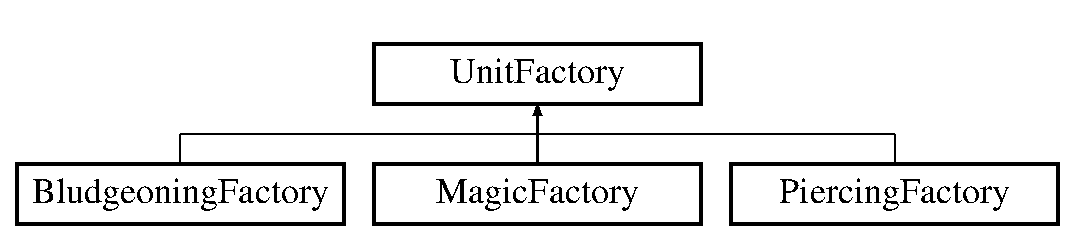
\includegraphics[height=2.000000cm]{class_unit_factory}
\end{center}
\end{figure}
\subsection*{Public Member Functions}
\begin{DoxyCompactItemize}
\item 
{\bf Unit} $\ast$ {\bfseries make\+Light} ()\label{class_unit_factory_a321efab812a837b52f303fc737048c30}

\item 
{\bf Unit} $\ast$ {\bfseries make\+Dark} ()\label{class_unit_factory_aa2f1d6eebffefbafa173b79fe38beb49}

\item 
virtual {\bf Unit} $\ast$ {\bfseries make\+Light} ()=0\label{class_unit_factory_a8857f9a5156d856c01dd95b58ff4133d}

\item 
virtual {\bf Unit} $\ast$ {\bfseries make\+Dark} ()=0\label{class_unit_factory_a14e80f213953ac2c4d58ea5d287762c4}

\end{DoxyCompactItemize}


\subsection{Detailed Description}
D\+O\+X\+Y\+G\+E\+N C\+O\+M\+M\+E\+N\+T H\+E\+R\+E. 

The documentation for this class was generated from the following files\+:\begin{DoxyCompactItemize}
\item 
Bludgeoning\+Factory.\+h\item 
Unit\+Factory.\+h\end{DoxyCompactItemize}

%--- End generated contents ---

% Index
\backmatter
\newpage
\phantomsection
\clearemptydoublepage
\addcontentsline{toc}{chapter}{Index}
\printindex

\end{document}
